\graphicspath{ {./assets/} }

\chapter{DNS szerver}

\section{Indítás}
Ahhoz, hogy használni tudjuk az email klienst, kritikus fontosságú a DNS szervernek a futtatása. Természetesen arra vonatkozik ez a megkötés, ha lokálisan futtatjuk az email szervert!
\begin{itemize}
    \item \verb|docker-compose up -d|
\end{itemize}

\begin{flushleft}
    Parancs futtatása után látható, hogy sikeresen elindult a DNS szerver.
    \begin{center}
        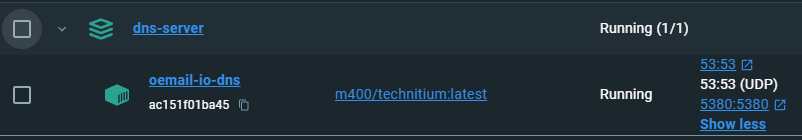
\includegraphics[width=0.9\textwidth]{docker-up-dns-server.png}
    \end{center}
\end{flushleft}

\section{Konfiguráció}
\begin{flushleft}
    Magát a konfigurációt webes környezetben hajthatjuk végre, amely látható is, hogy a \textbf{5380} porton fut. Cím, amelyen a konfigurációt elvégezhetjük:
    \begin{itemize}
        \item \verb|http://localhost:5380/|
    \end{itemize}
\end{flushleft}

\subsection{Zóna hozzáadása}
Megadott paraméterek:
\begin{itemize}
    \item Zóna neve: \verb|oemail.io|
    \item Típus: \verb|Primary Zone|
\end{itemize}

\subsection{Rekordok hozzáadása}
\begin{flushleft}
    Korábban létrehozott \verb|oemail.io| zónához rekordok hozzáadása szükséges az email szerverhez.
\end{flushleft}
\begin{itemize}
    \item \verb|MX| típusú rekord paraméterei:
    \begin{itemize}
        \item Name: \verb|@| (rámutat az aktuális DNS rekordra)
        \item TTL: \verb|3600| (1 óra)
        \item Preference: \verb|10|
        \item Exchange: \verb|mail.oemail.io|
    \end{itemize}
    \item \verb|A| típusú rekord paraméterei:
    \begin{itemize}
        \item Name: \verb|mail|
        \item TTL: \verb|3600| (1 óra)
        \item IPv4 Address: \verb|127.0.0.1|
    \end{itemize}
\end{itemize}
\subsection{Tesztelés nslookup parancs segítségével}
Az alábbi parancs segítségével tesztelhetjük a korábban beállított paramétereket: \verb|nslookup mail.oemail.io|
\begin{flushleft}
    MX rekord paraméterek ellenőrzése: \verb|nslookup -type=mx oemail.io 127.0.0.1|
\end{flushleft}